\documentclass[english, a4paper,11pt]{article}
\usepackage[latin1]{inputenc}
\usepackage[T1]{fontenc}
\usepackage{bbm}
\usepackage{amsmath}
\usepackage{indentfirst}
\usepackage{fullpage}
\usepackage{url}
\usepackage{graphicx}
\usepackage{geometry}
\geometry{verbose,tmargin=3cm,bmargin=2cm,lmargin=2cm,rmargin=2cm}
\usepackage{babel}
\usepackage[center,footnotesize]{caption}
\usepackage[section]{placeins}
\usepackage{subfig}
\title{Solutions - Series 3}
\date{October 9, 2012}
\author{Genomics and bioinformatics - Week 4}
\begin{document}
\maketitle

\section{Global alignment}
\subsection{The table}
\noindent
Using the given scoring matrix $M$, one deduces the following rules to compute the 3 intermediate scores in each cell:
\begin{itemize}
\item Upper neighbour cell score - 2
\item Left neighbour cell score - 2
\item Upper-left neighbour cell score $\left\{\begin{array}{l} +1 \mbox{ if nucleotides are identical} \\ -1 \mbox{ if nucleotides are different}\end{array} \right.$
\end{itemize}
The highest score is then retained and the corresponding arrow is labelled. Here is the resulting table: \\
\begin{center}
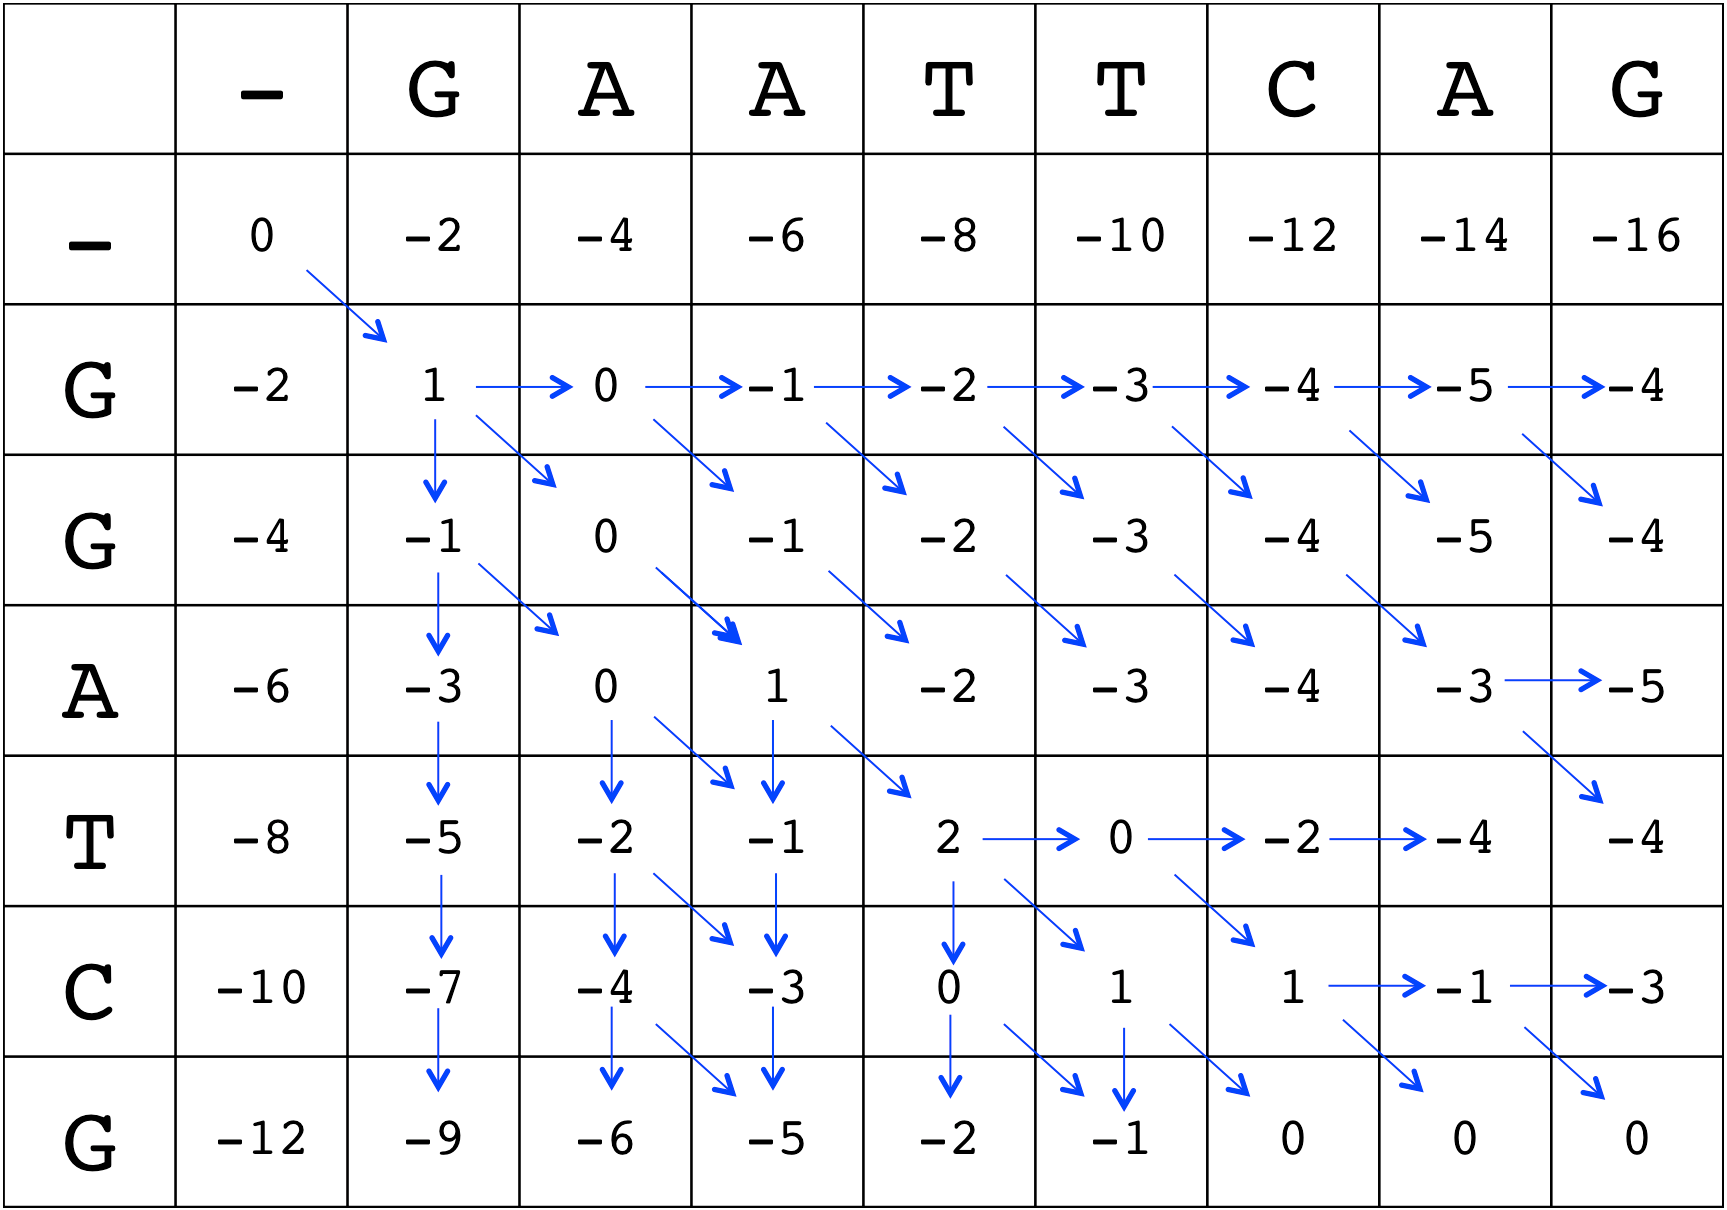
\includegraphics[width=0.6\textwidth]{scoring.png}\\
\end{center}

\subsection{Backtracking}
\noindent
One then applies the traceback process to the obtained table to deduce the best alignment between the two reads. 
The traceback begins with the bottom-right cell and is completed when the top-left cell of table is reached. Note that several 
traceback paths are possible and thus in general there may be more than one optimum alignment. The best alignments are given by the paths that have the maximum score. A traceback path is highlighted below.

\begin{center}
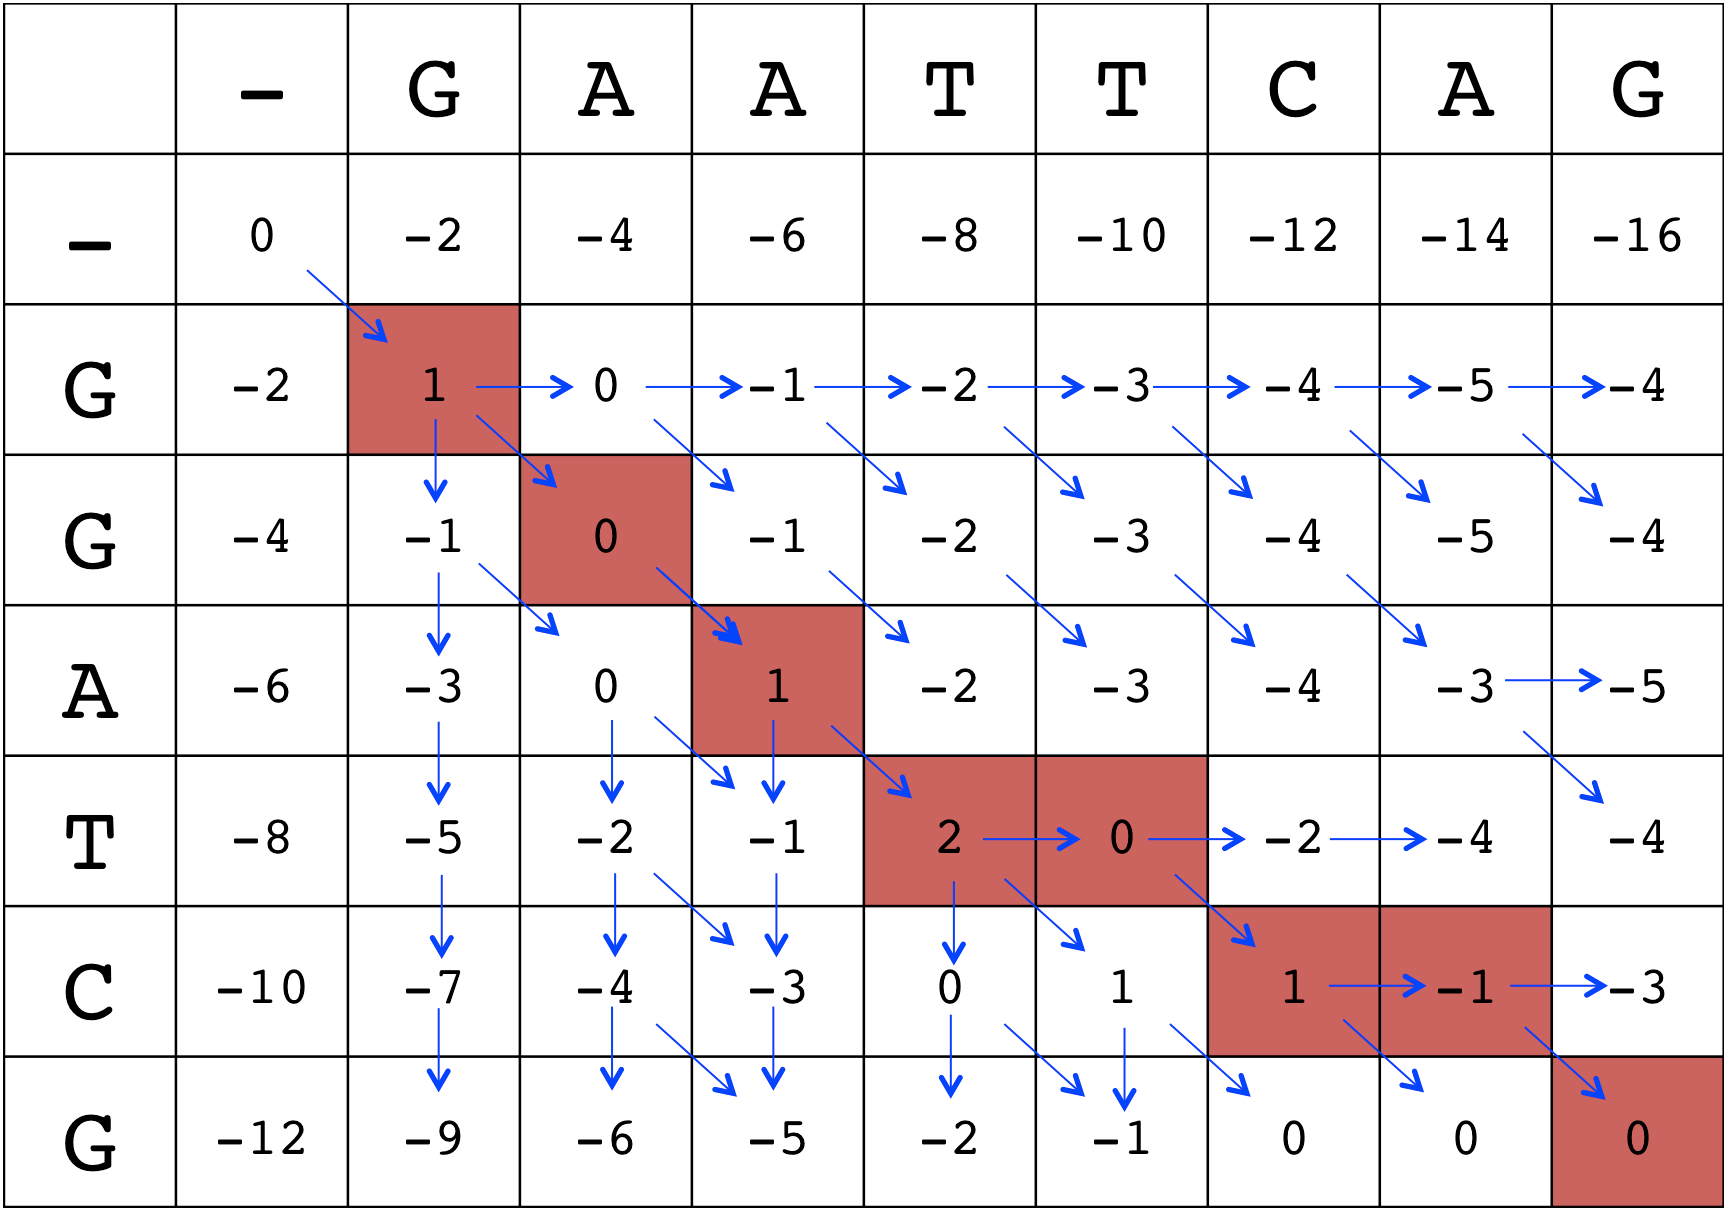
\includegraphics[width=0.6\textwidth]{backtracking.png}
\end{center}

\subsection{Alignment}
\noindent
An optimal alignment is easily obtained by using the following arrow rules:
\begin{center}
Left/Right = Deletion, Up/Down = Insertion, and Diagonal = Match.
\end{center}
An optimal alignment is

\begin{center}
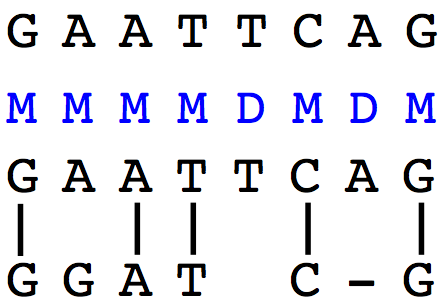
\includegraphics[width=0.2\textwidth]{alignment.png}
\end{center}



\section{HMM}

\subsection{Finding the Emission and Transition Probabilities}
The corresponding HMM is described in the following figure:


\begin{centering}
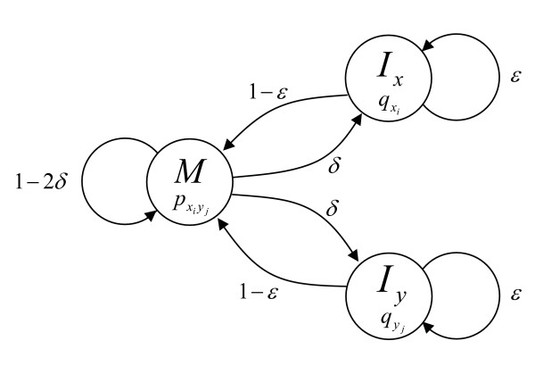
\includegraphics[width=0.3\textwidth]{HMM.jpg}

\end{centering}

\begin{enumerate}
\item Transitions: from $d = log_2(\delta)$ and $d = -2$ we deduce $\delta = 2^{-2} = \frac{1}{4} = \varepsilon$.
\item Emissions: $p(x)$ is the probability of choosing one nucleotide at random: $p(x)=p(y)=1/4$.\\
Inverting the formula for $S(x,y)$, one gets $p(x,y) = \frac{1}{16}2^{S(x,y)}$: \\
$p(x,x) = \frac{1}{8}$,\\
$p(x,y) = \frac{1}{32}$ if $x \neq y$.
\end{enumerate}

\subsection{Constructing the Three Matrices (VM,VD and VI)}

Then we can construct the three matrices for VM, VD and VI by the Viterbi algorithm.

Matrix $V_M$:
%\begin{figure}[h]
\begin{center}
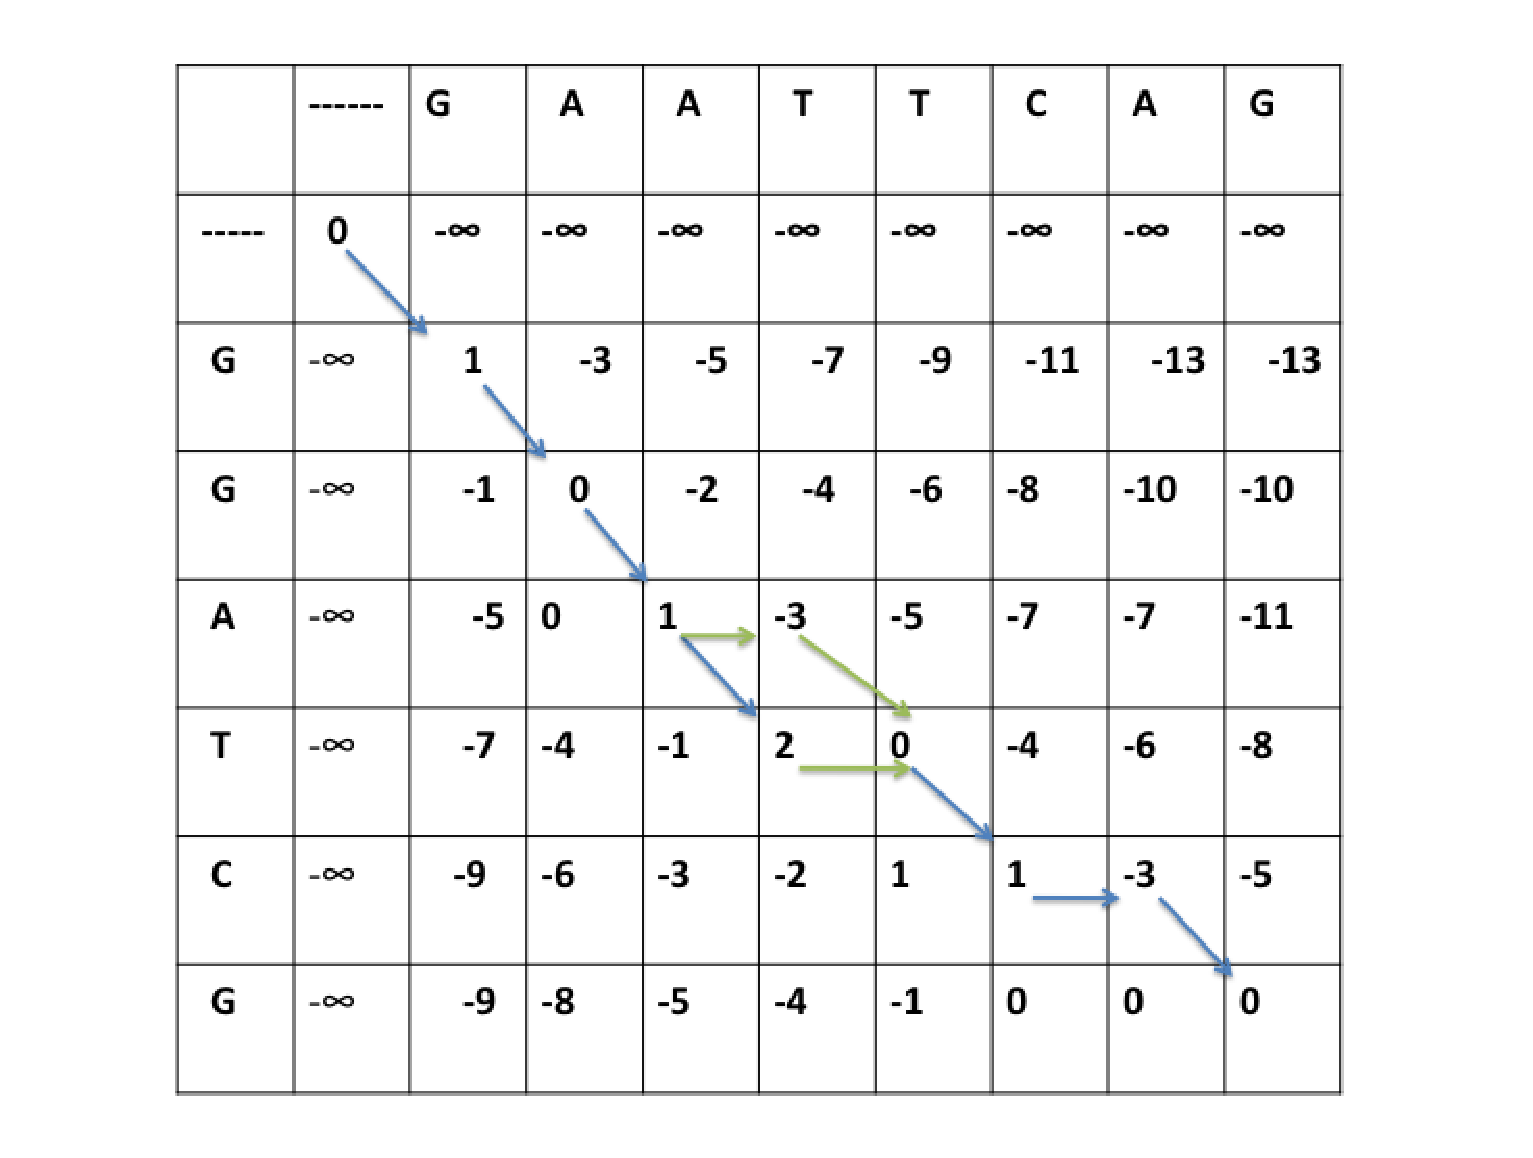
\includegraphics[width=0.8\textwidth]{Slide1.eps}
%\caption{The matrix for the match state VM}
\end{center}
%\end{figure}

\newpage
Matrix $V_D$:
%\begin{figure}[h]
\begin{center}
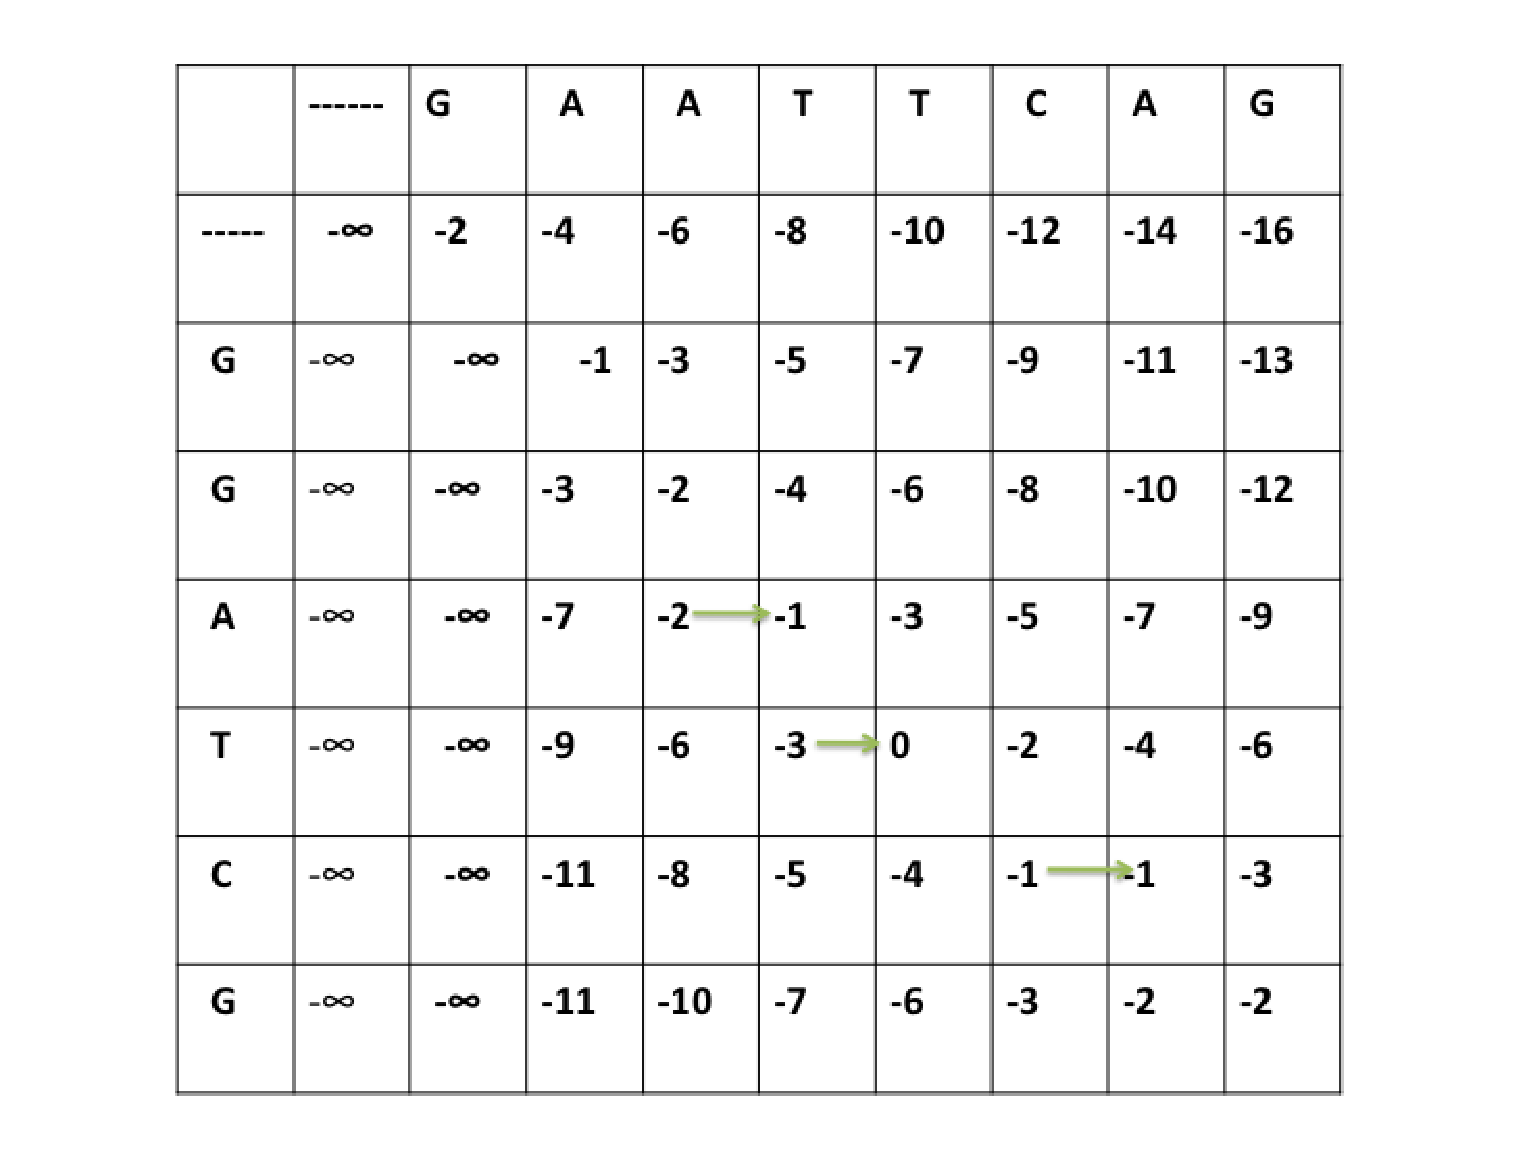
\includegraphics[width=0.8\textwidth]{Slide2.eps}
%\caption{Matrix for deletion state VD}
\end{center}
%\end{figure}

Matrix $V_I$:
%\begin{figure}[h]
\begin{center}

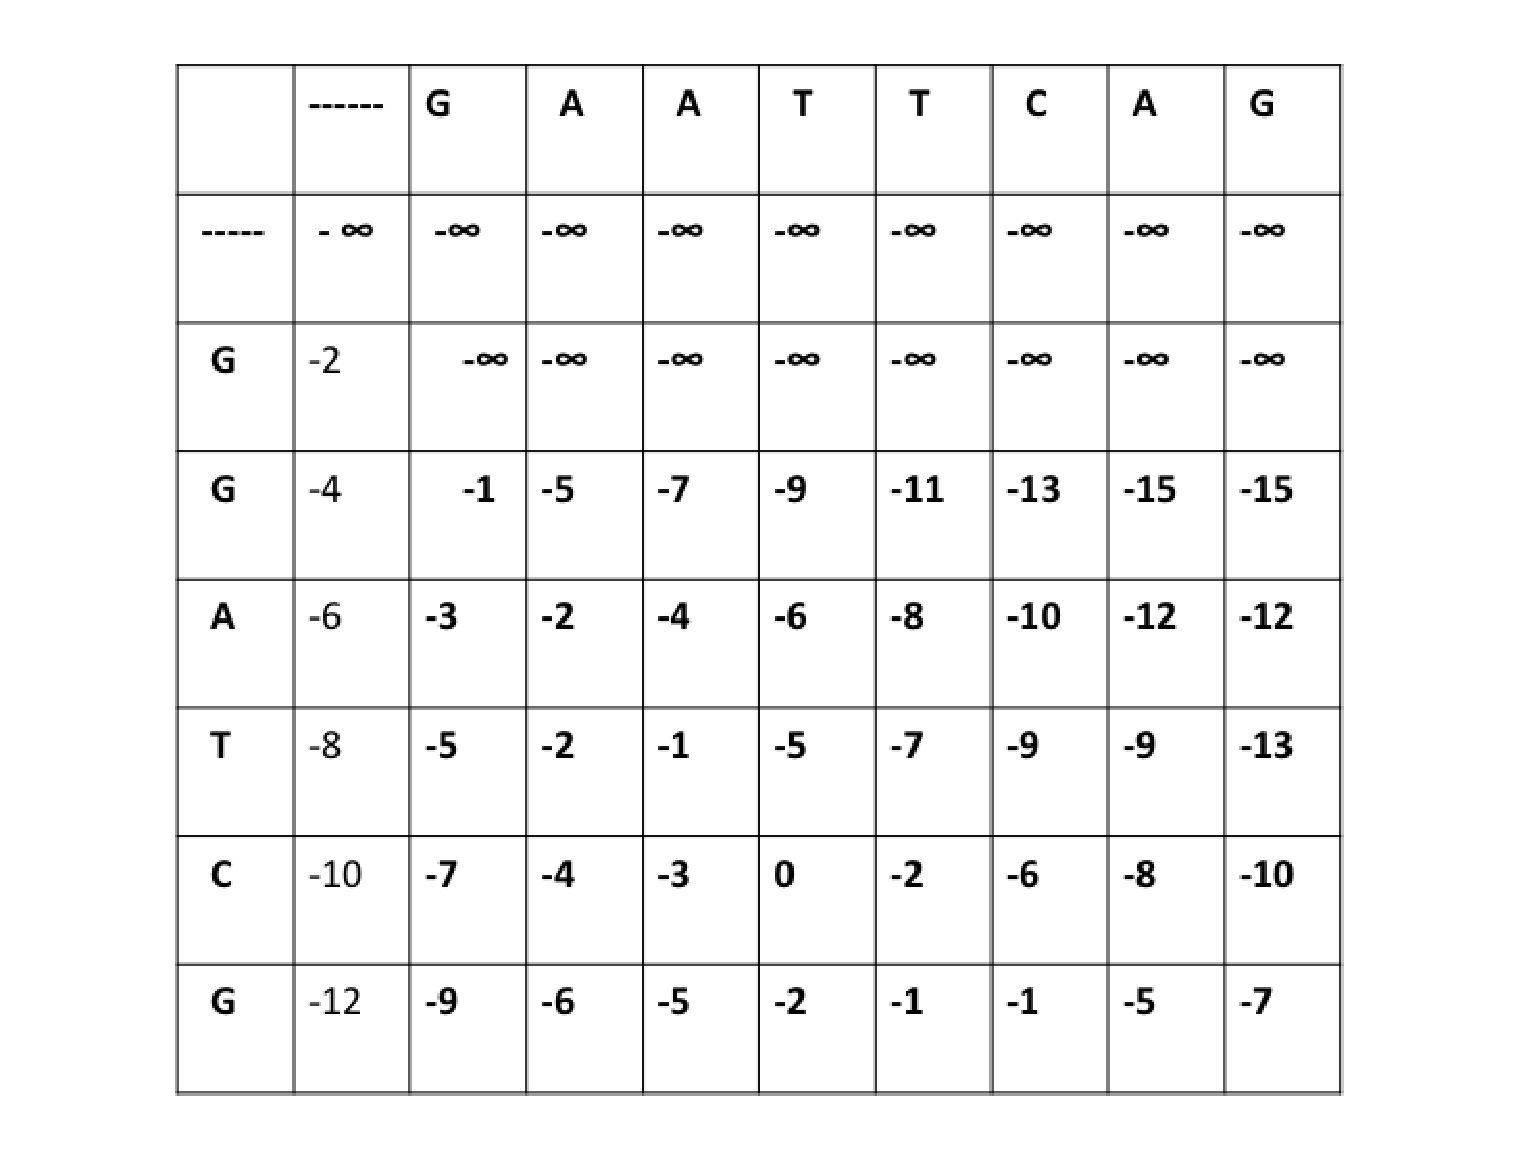
\includegraphics[width=0.8\textwidth]{Slide3.eps}
%\caption{Matrix for insertion state VI}
\end{center}
%\end{figure}

\subsection{Deducing the Alignments}

The final matrix is formed by taking maximum value from the three elements of each matrix.
\newpage
Alignment by backtracking:
%\begin{figure}[ht]
\begin{center}
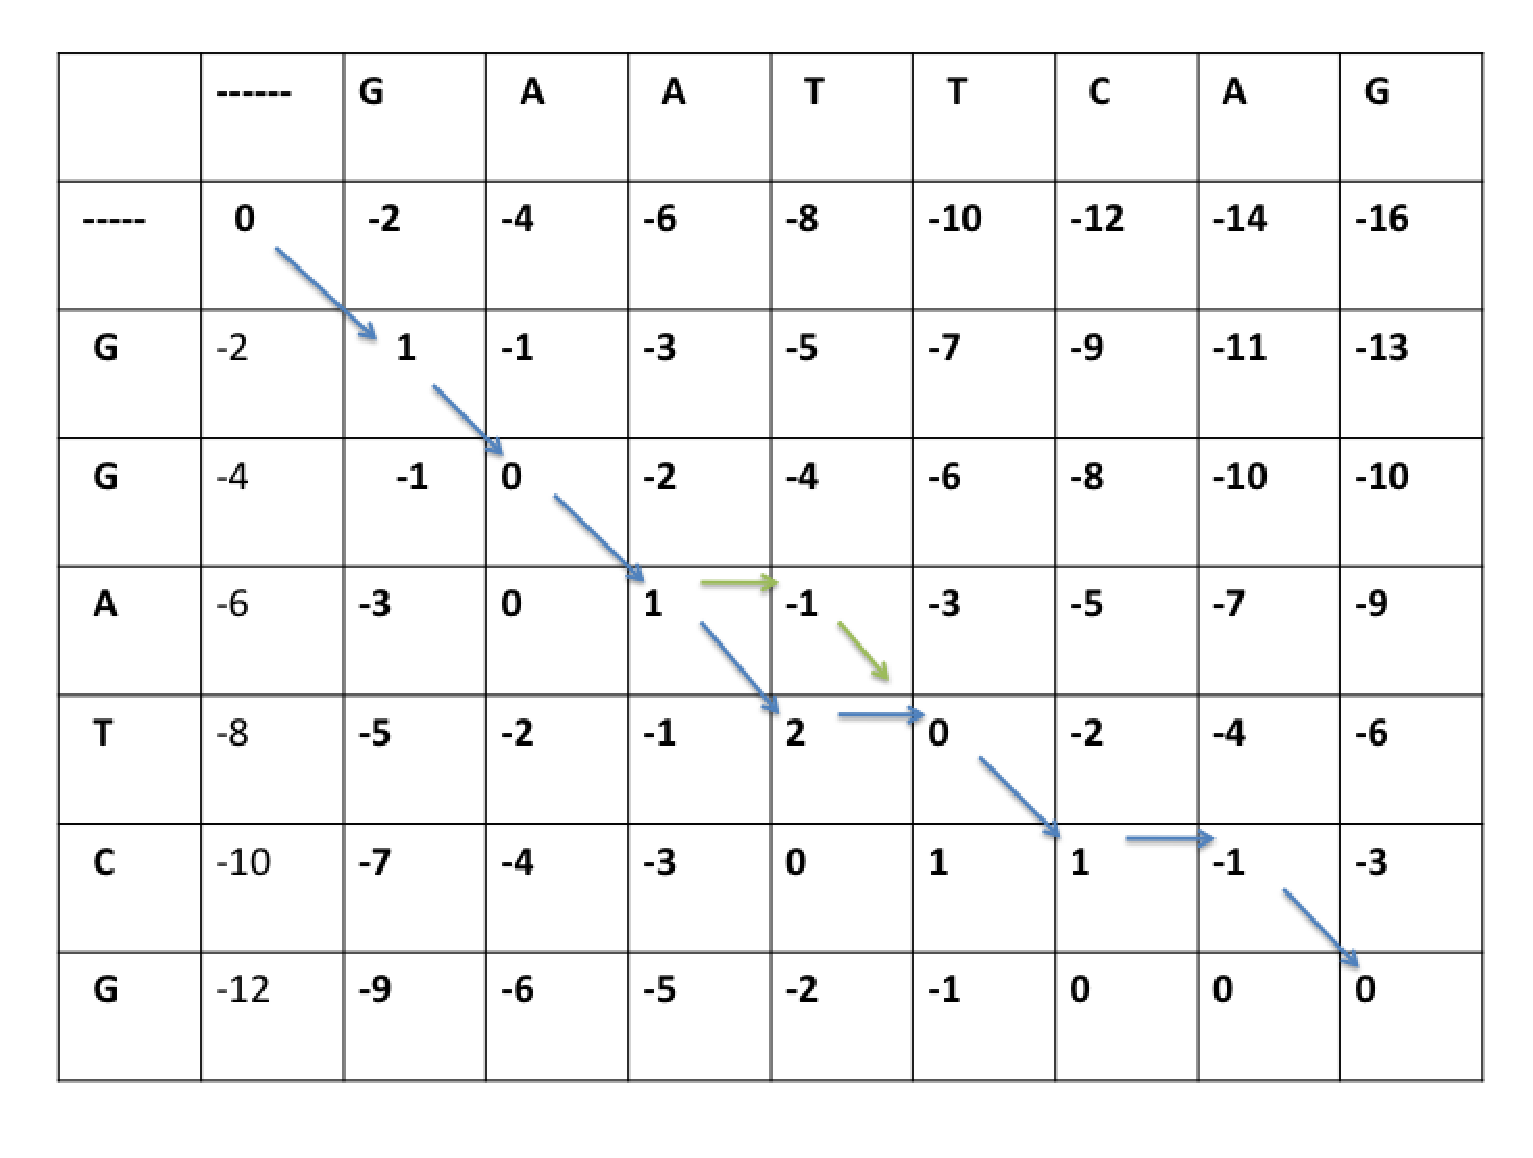
\includegraphics[width=0.6\textwidth]{Slide4.eps}
%\caption{Alignment by backtracking}
\end{center}
%\end{figure}

There are two possible optimal alignments.

%\begin{figure}[h]
\begin{center}
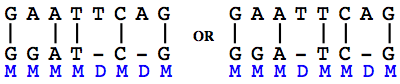
\includegraphics[width=0.6\textwidth]{alignment2.png}
\end{center}
%\caption{The alignments}
%\end{figure}

\end{document}
